% !TeX program = xelatex
\documentclass{anisyan-resume}

%--------------------
%      Packages
%--------------------
\usepackage[utf8]{inputenc}
\usepackage{adjustbox}
\usepackage{amssymb}
\usepackage{graphicx}
\usepackage{caption}
\usepackage{subcaption}
\usepackage{array}
\usepackage{makecell}
\usepackage[top=5mm,
	bottom=5mm,
	left=5mm,
	right=10mm]{geometry}
\usepackage{fontawesome}
\usepackage{xcolor}
\usepackage{setspace}
\usepackage[colorlinks = true,
	linkcolor = blue,
	urlcolor  = blue,
	citecolor = blue,
	anchorcolor = blue]{hyperref}
\usepackage{multirow}
\usepackage{tabularx}
\usepackage{enumitem}
\usepackage{fontspec}
\setmainfont{Arial}

\begin{document}
	%--------------------
	%      HEADER
	%--------------------
	\begin{tabular}{ m{4cm} t{9cm} m{5cm} }
		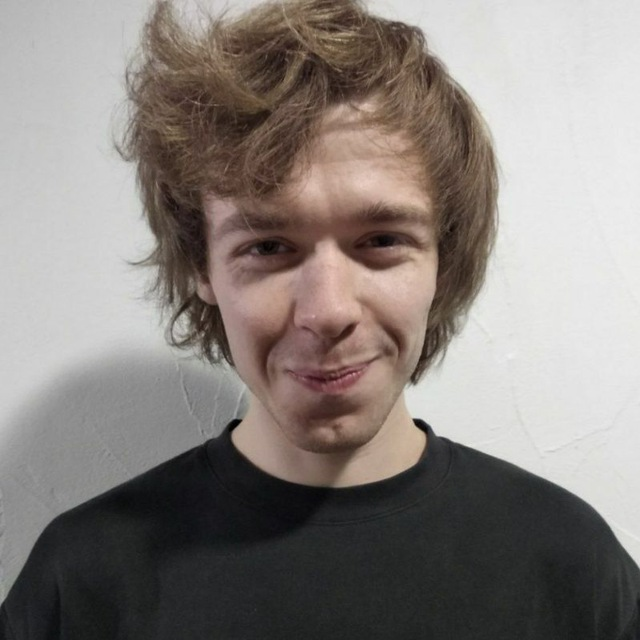
\includegraphics[width=4cm, height=4cm]{avatar1.jpg}
		&
		\begin{tabular}{ m{9cm} }
			\textbf{\Huge Aleksandr Anisimov} \\
			\Large {Embedded Software Engineer} \\
			\Large {with Laser Physics background} \\
			\vspace{1cm}
			\large{Looking for a PhD in Laser or Plasma} \\
			\large{Physics related position.}
		\end{tabular}
		&
		\makepersonallinks{375257152681}
		 					{+375(25)-715-26-81}
		 					{anisimov.alexander.s}
		 					{https://github.com/anisyanka}
		 					{https://www.linkedin.com/in/anisyanka/}
		 					{https://stackoverflow.com/users/9308555/anisyanka}
	\end{tabular}

	%--------------------
	%      SKILLS
	%--------------------
	\vspace{5pt}
	\section{\textbf{SKILLS}}
	\vspace{5pt}
	\def\arraystretch{1.2}
	\begin{tabular}{ >{\quad}l p{12.5cm} }
		\normalsize\textbf{Basis} & \normalsize{Laser physics, Plasma, Interferometry, Laser Doppler velocimetry} \\
		\normalsize\textbf{Programming languages} & \normalsize{С/C++, Bash, Python, HTML, CSS, JavaScript, SQL} \\
		\normalsize\textbf{Hardware} & \normalsize{STM32, NRF52 BLE, 8051 core, ESP32, st-link, Trace-32} \\
		\normalsize\textbf{Other} & \normalsize{GNU make, Git, Vim, Markdown, \LaTeX, RPM spec} \\
		\normalsize\textbf{Keywords} & \normalsize{SSD, microcontrollers, DSP, ARM, TrustZone, REE, TEE, Linux kernel, LDD} \\
	\end{tabular}

	%--------------------
	%      EDUCATION
	%--------------------
	\vspace{5pt}
	\section{\textbf{EDUCATION}}
	\vspace{5pt}
	\def\arraystretch{1.2}
	\begin{tabular}{ m{20cm} }
		\quad\href{https://eng.mephi.ru/}{\large \textbf{National Research Nuclear University MEPhI}} \\
		\quad\normalsize{\textbf{Bachelor's degree}, laser fusion, sept. 2013 - june 2017} \\
		\quad\small\textbf{Diploma: } \small{Development of a multichannel system for photoelectric conversion of signals for laser interferometer of the VISAR type} \\
		\renewcommand\labelitemi{{\boldmath$\cdot$}}
			\begin{itemize}[noitemsep, topsep=5pt, parsep=0pt, partopsep=0pt]
				\addtolength{\itemindent}{40pt}
				\item {\small Measurement velocity of shock wave in solid state}
				\item {\small Development firmware to adjust the intensity of light entering the photodetector}
			\end{itemize}

		\vspace{5pt}

		\quad\normalsize{\textbf{Master's degree}, embedded systems, sept. 2017 - june 2019} \\
		\quad\small\textbf{Diploma: } \small{Development of a training course on the application of DSP-processors for digital signal processing tasks} \\
		\renewcommand\labelitemi{{\boldmath$\cdot$}}
		\begin{itemize}[noitemsep, topsep=5pt, parsep=0pt, partopsep=0pt]
			\addtolength{\itemindent}{40pt}
			\item {\small Implement hardware drivers for Russian DSP processor}
			\item {\small Implement DSP algorithms: digital filters, Fourier analysis}
		\end{itemize}
	\end{tabular}

	%--------------------
	%      WORK EXPERIENCEE
	%--------------------
	\vspace{5pt}
	\section{\textbf{WORK EXPERIENCE}}
	\vspace{5pt}
	\renewcommand\arraystretch{0.5}
	\begin{tabularx}{\textwidth}{>{\quad}m{4cm} | @{\timelinebullet} l}
		% SK Hynix
		%-------------------------------------------------------------------------------------------
		\normalsize\textbf{Now 2021 -- Now}
		&
		\renewcommand\arraystretch{1}
		\begin{tabular}[t]{ p{15cm} }
		\large{\textbf{SSD Firmware Development Engineer}} \texttt{\textbf{@}}\href{https://skhms.by/en/sk-hynix-development-center-in-minsk/}{\textbf{SK Hynix}}\\
		\normalsize{Memory solutions}
		\renewcommand\labelitemi{{\boldmath$\cdot$}}
			\begin{itemize}[noitemsep, topsep=5pt, parsep=0pt, partopsep=0pt]
				\item {\small Implement NVMe SSD firmware layers (HIL/FTL/FIL) in C/C++}
				\item {\small Implement firmware test code for regression failures/corner cases troubleshooting}
				\item {\small Perform firmware code review and improvement}
				\item {\small Perform firmware failure analysis and corrective actions applying}
			\end{itemize}
		\end{tabular} \\

		% OMP
		%-------------------------------------------------------------------------------------------
		\normalsize\textbf{Jul 2019 -- Nov 2021}
		&
		\renewcommand\arraystretch{1}
		\begin{tabular}[t]{ p{15cm} }
			\large{\textbf{System Software Engineer}} \texttt{\textbf{@}}\href{https://auroraos.ru/}{\textbf{Aurora OS}} \\
			\normalsize{Mobile OS based on Linux}
			\renewcommand\labelitemi{{\boldmath$\cdot$}}
			\begin{itemize}[noitemsep, topsep=5pt, parsep=0pt, partopsep=0pt]
				\item {\small Development TEE side of Russian fork of Sailfish OS (Aurora OS)}
				\item {\small Development hardware-backed keystore and trusted services}
				\item {\small Designed new features for Linux kernel OP-TEE driver for in-house Linux distro}
				\item {\small CVE fixing for government certification (FSTEK Russia)}
				\item {\small Took part in preparation solution for \href{https://github.com/OP-TEE/optee_os/issues/4230}{TEE logger}}
			\end{itemize}
		\end{tabular} \\

		% Yandex
		%-------------------------------------------------------------------------------------------
		\normalsize\textbf{Sept 2018 -- Mar 2019}
		&
		\renewcommand\arraystretch{1}
		\begin{tabular}[t]{ p{15cm} }
			\large{\textbf{Embedded Software Engineer}} \texttt{\textbf{@}}\href{https://en.wikipedia.org/wiki/Yandex}{\textbf{Yandex}}\\
			\normalsize{Self-driving cars}
			\renewcommand\labelitemi{{\boldmath$\cdot$}}
			\begin{itemize}[noitemsep, topsep=5pt, parsep=0pt, partopsep=0pt]
				\item {\small Development emergency stop button for self-driving cars (FreeRTOS, STM32, CAN, radio module)}
				\item {\small Reverse engineering for update protocol for radio modules to update its firmware by other chip}
				\item {\small Development from scratch driver for SPI-based e-paper displays}
				\item {\small Writing unit-tests with cpputest for main board in a car}
			\end{itemize}
		\end{tabular} \\

		% SmartAirkey
		%-------------------------------------------------------------------------------------------
		\normalsize\textbf{Feb 2018 -- Sept 2018}
		&
		\renewcommand\arraystretch{1}
		\begin{tabular}[t]{ p{15cm} }
			\large{\textbf{Embedded Software Engineer}} \texttt{\textbf{@}}\href{https://smartairkey.com/en/}{\textbf{SmartAirkey}}\\
			\normalsize{Wireless solutions startup}
			\renewcommand\labelitemi{{\boldmath$\cdot$}}
			\begin{itemize}[noitemsep, topsep=5pt, parsep=0pt, partopsep=0pt]
				\item {\small Development firmware for a Bluetooth-lock based on Nordic BLE stack and FreeRTOS}
				\item {\small Soldering and testing boards}
			\end{itemize}
		\end{tabular} \\

	\end{tabularx}

	\newpage 

	\vspace*{25pt}
	
	\begin{tabularx}{\textwidth}{>{\quad}m{4cm} | @{\timelinebullet} l}
		
		% Amplituda
		%-------------------------------------------------------------------------------------------
		\normalsize\textbf{Sept 2016 -- Feb 2018}
		&
		\renewcommand\arraystretch{1}
		\begin{tabular}[t]{ p{15cm} }
			\large{\textbf{Junior Embedded Engineer}} \texttt{\textbf{@}}\href{http://www.amplituda.ru/}{\textbf{Amplituda}}\\
			\normalsize{Radiation safety technologies}
			\renewcommand\labelitemi{{\boldmath$\cdot$}}
			\begin{itemize}[noitemsep, topsep=5pt, parsep=0pt, partopsep=0pt]
				\item {\small Development firmware for $\gamma$-sensors based on RS-485 and stm32f103}
				\item {\small Development low-level drivers for ADC, DAC, OLED, touchscreens, RTC, USB, DHT11, HD44780 etc}
			\end{itemize}
		\end{tabular}		
	\end{tabularx}

	%--------------------
	%      ACHIEVEMENTS
	%--------------------
	\section{\textbf{ACHIEVEMENTS}}
	\vspace{5pt}
	\begin{itemize}[noitemsep, topsep=5pt, parsep=0pt, partopsep=0pt]
		\item {\small{Fix CVE-2020-6096 in GNU C Library for ARMv7 memcpy(). More info: 	[\href{https://sourceware.org/pipermail/libc-alpha/2020-June/114702.html}{link1}],
			[\href{https://sourceware.org/pipermail/libc-alpha/2020-June/114919.html}{link2]},
			[\href{https://sourceware.org/pipermail/libc-alpha/2020-July/115923.html}{link3]},
			[\href{https://sourceware.org/pipermail/libc-alpha/2020-July/115924.html}{link4]}}}
		\item {\small{Loadable plugin framework in OP-TEE project. More info:
		[\href{https://github.com/OP-TEE/optee_client/issues/219}{link1}],
			[\href{https://github.com/OP-TEE/optee_client/pull/239}{link2]},
			[\href{https://github.com/OP-TEE/optee_os/pull/4248}{link3]},
			[\href{https://github.com/linaro-swg/optee_examples/pull/79}{link4]},
			[\href{https://github.com/OP-TEE/optee_test/pull/482}{link5]},
			[\href{https://github.com/OP-TEE/optee_docs/pull/102}{link6}]}}
	\end{itemize}
\end{document}
Loadable plugin framework in OP-TEE project [link1], [link2], [link3], [link4], [link5]
